\documentclass[11pt,a4paper]{article}

\usepackage[margin=1in]{geometry}
\usepackage{amsmath,amssymb}
\usepackage{graphicx}
\usepackage{booktabs}
\usepackage{hyperref}
\usepackage{xcolor}
\usepackage{caption}
\usepackage{subcaption}
\usepackage{enumitem}
\usepackage{parskip}
\usepackage{microtype}
\usepackage{float}

\hypersetup{colorlinks=true, linkcolor=blue, citecolor=blue, urlcolor=blue}

\title{\textbf{AE646 --- Interim Report (Stage 2)}\\[0.5em]
\large Operator Learning for Parametric Darcy Flow: FNO vs.\ MLP Baseline}
\author{Team PINNacles\\Aryamann Srivastava\\Department of Aerospace Engineering, IIT Kanpur}
\date{September 2026}

\begin{document}
\maketitle

% ─────────────────────────────────────────────────────────────────────────────
\section{Introduction and Motivation}

Traditional numerical solvers such as Finite Difference Methods (FDM) and Finite Element Methods (FEM) require re-solving the full PDE for every new set of parameters, imposing prohibitive computational cost when thousands of queries are needed (e.g., uncertainty quantification, inverse design, real-time control). Neural operators learn a mapping between infinite-dimensional function spaces and amortise this cost over many queries.

This project evaluates two architectures for the 2D parametric Darcy flow problem:
\begin{itemize}[nosep]
  \item \textbf{MLP baseline} --- a fully-connected network with no structural inductive bias.
  \item \textbf{Fourier Neural Operator (FNO)} \cite{li2021fno} --- a resolution-invariant architecture whose trainable weights reside in the frequency domain.
\end{itemize}

Both are trained to map the permeability field $\kappa(x,y)$ and spatial coordinates $(x,y)$ to the pressure field $u(x,y)$ satisfying the 2D Darcy equation:
\begin{equation}
  -\nabla \cdot (\kappa(x,y)\,\nabla u(x,y)) = f(x,y), \quad (x,y)\in[0,1]^2,
  \label{eq:darcy}
\end{equation}
with homogeneous Dirichlet boundary conditions. The forcing $f = 1$ is constant; the permeability $\kappa \in \{0.1, 1.0\}$ is piecewise-constant, randomly distributed on a $64\times 64$ grid.

% ─────────────────────────────────────────────────────────────────────────────
\section{Dataset Setup}

\subsection{Source}
We use the PDEBench dataset \cite{takamoto2022pdebench} (DOI: \texttt{10.18419/darus-2986}), a benchmark suite for scientific machine learning. The 2D Darcy flow split provides 10\,000 samples at $128\times128$ resolution.

\subsection{Preprocessing}
Each sample consists of:
\begin{itemize}[nosep]
  \item \textbf{Input}: $\kappa(x,y)$ subsampled from $128\times128$ to $64\times64$ by taking every second grid point (literature-standard subsampling; PDEBench's own loaders do the same).
  \item \textbf{Grid coordinates}: $(x,y)\in[0,1]^2$ concatenated channel-wise to give a 3-channel input tensor of shape $64\times64\times3$.
  \item \textbf{Target}: pressure $u(x,y)$ at $64\times64$.
\end{itemize}

From the 10\,000-sample archive we draw a reproducible (seed 42), non-overlapping subset: a 1\,000-sample train/val pool --- split 900 train / 100 validation --- and 200 further samples held out entirely throughout training and used only for final evaluation. These counts match those used in the original FNO work (Li et al.\ 2021), so our numbers are directly comparable to the literature. Data are loaded in mini-batches of 16 and normalised with training-set statistics only.

\subsection{Why Only a 1\,000-Sample Training Pool?}
The original FNO Darcy experiments use $\sim$1\,000 training samples; matching this keeps the comparison with published numbers clean and the training cost modest. 100 validation samples give a stable loss estimate for checkpoint selection, and the 200-sample test set is large enough for generalisation statistics with standard error $\lesssim 0.003$.

% ─────────────────────────────────────────────────────────────────────────────
\section{Model Architectures}

\subsection{MLP Baseline}
The MLP baseline flattens the $64\times64\times3$ input into a vector of 12\,288 features and applies three hidden layers of width 2048 with GELU activations:
\[
  \text{MLP}: \mathbb{R}^{12288} \xrightarrow{2048} \xrightarrow{2048} \xrightarrow{2048} \mathbb{R}^{4096} \to \mathbb{R}^{64\times64},
\]
with a final linear projection. Total parameters: $\approx 42$\,M. The MLP is fixed to the training resolution ($64\times64$) and cannot generalise to other grid sizes.

\subsection{Fourier Neural Operator (FNO)}
The FNO \cite{li2021fno} processes the input as a $64\times64\times3$ field tensor through five stages:
\begin{enumerate}[nosep]
  \item \textbf{Lifting}: a pointwise linear layer maps 3 input channels to 64 hidden channels.
  \item \textbf{Four Spectral Convolution Blocks}: each block computes (i) a 2D FFT of the 64-channel field, (ii) retains only the lowest 12 Fourier modes in each direction ($12\times12$ complex-valued coefficients), (iii) multiplies by learned complex weights of shape $64\times64\times12\times12$, (iv) applies an inverse FFT, and (v) adds a pointwise local convolution bypass (equivalent to a $1\times1$ convolution).
  \item \textbf{Projection}: two linear layers ($64\to128\to1$) map hidden channels to the scalar output.
\end{enumerate}
Because the learned weights operate in frequency space (not on a fixed grid), the same trained network can be evaluated at any grid resolution --- the key property exploited in our zero-shot super-resolution experiments (Section~\ref{sec:superres}). Total parameters (baseline config): $\approx 4.7$\,M.

% ─────────────────────────────────────────────────────────────────────────────
\section{Training Protocol}

Both models are trained with:
\begin{itemize}[nosep]
  \item \textbf{Loss}: Relative $L_2$ error $\|{\hat{u} - u}\|_2 / \|{u}\|_2$ per sample, averaged over the batch.
  \item \textbf{Optimiser}: Adam, learning rate $10^{-3}$, cosine annealing schedule (min LR $10^{-5}$).
  \item \textbf{Batch size}: 16; up to 100 epochs (200 for the larger FNO-improved configuration). No early stopping --- every run completes its full epoch budget and the checkpoint with the lowest validation relative-$L_2$ error is retained.
  \item \textbf{Hardware}: NVIDIA RTX PRO 6000 (CUDA), PyTorch 2.x.
\end{itemize}

\subsection{FNO Improved Configuration}
An extended FNO configuration (\texttt{fno\_improved}) was also trained with doubled width (128 channels), more Fourier modes (20 per direction, up from 12), and 6 spectral blocks (up from 4), totalling $\approx78.8$\,M parameters. This represents a scaling experiment to probe the accuracy--parameter trade-off.

% ─────────────────────────────────────────────────────────────────────────────
\section{Preliminary Quantitative Results}

All metrics are computed on the held-out 200-sample test set. Error is relative $L_2$: $\epsilon_{\rm rel} = \|{\hat{u} - u}\|_2 / \|{u}\|_2$.

\begin{table}[H]
\centering
\caption{Test-set performance at training resolution ($64\times64$). Lower is better.}
\label{tab:results}
\begin{tabular}{lrrrrrr}
\toprule
Model & Params & Mean & Median & Std & Min & Max \\
\midrule
MLP baseline   & 42.0\,M & 0.0820 & 0.0695 & 0.0456 & 0.0325 & 0.3367 \\
FNO original   &  4.7\,M & 0.0521 & 0.0398 & 0.0451 & 0.0155 & 0.3467 \\
FNO improved   & 78.8\,M & \textbf{0.0456} & \textbf{0.0307} & 0.0487 & \textbf{0.0106} & 0.3535 \\
\bottomrule
\end{tabular}
\end{table}

Key observations:
\begin{enumerate}[nosep]
  \item The FNO original achieves $37\%$ lower mean error than the MLP while using $9\times$ fewer parameters, demonstrating the advantage of spectral inductive biases for smooth PDE solutions.
  \item FNO improved reduces mean error a further $12\%$ over FNO original, at the cost of a $17\times$ parameter increase --- indicating diminishing returns in the scaling regime tested.
  \item All models exhibit right-skewed distributions: most samples have errors well below 0.1, but a small fraction ($\lesssim5\%$) with highly heterogeneous $\kappa$ fields drive errors toward 0.3 (see Figure~\ref{fig:hist}).
\end{enumerate}

\begin{figure}[H]
\centering
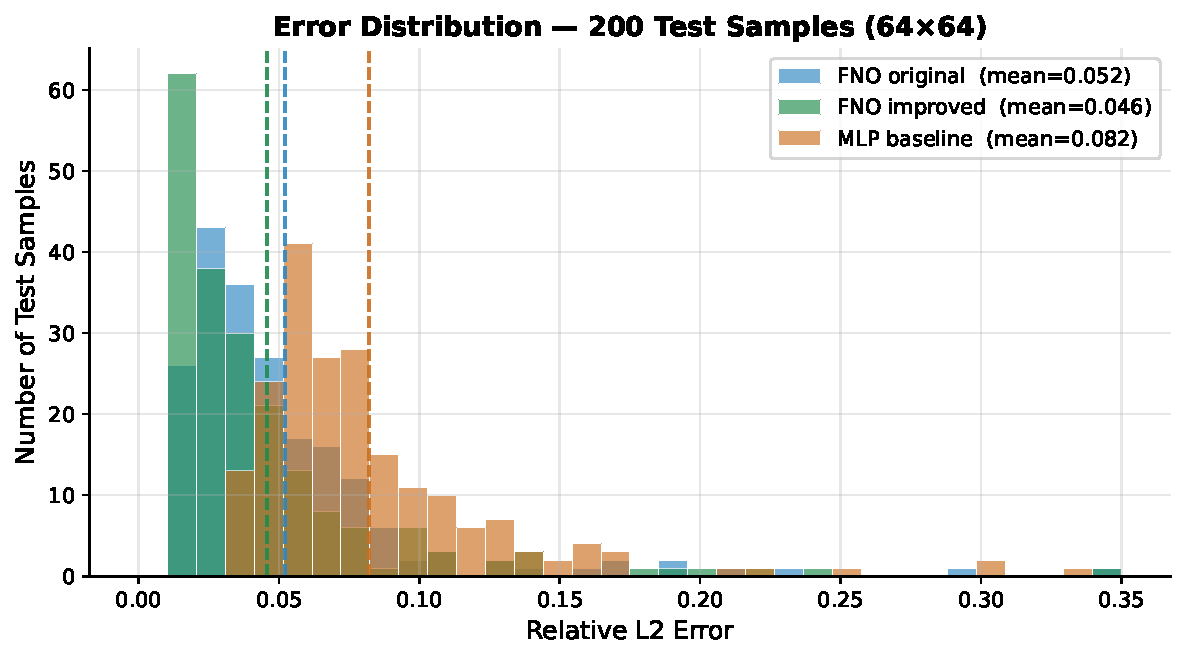
\includegraphics[width=0.62\textwidth]{../results/figures/fig1_error_histogram.pdf}
\caption{Error distribution across 200 test samples. Dashed vertical lines indicate per-model means. FNO errors are concentrated at lower values; MLP's distribution is shifted right.}
\label{fig:hist}
\end{figure}

\begin{figure}[H]
\centering
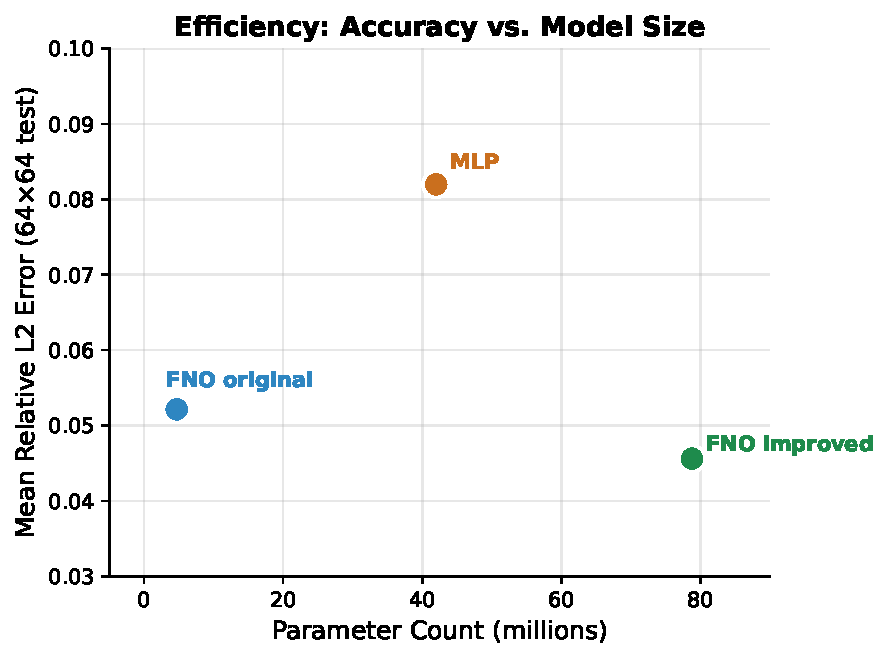
\includegraphics[width=0.55\textwidth]{../results/figures/fig2_efficiency_scatter.pdf}
\caption{Accuracy--efficiency scatter: FNO original occupies the favourable lower-left region (high accuracy, low parameter count). Scaling FNO to 78.8\,M params yields only marginal accuracy gain.}
\label{fig:scatter}
\end{figure}

% ─────────────────────────────────────────────────────────────────────────────
\section{Zero-Shot Super-Resolution}
\label{sec:superres}

Because FNO's spectral weights are resolution-agnostic, the same trained model can be queried on a finer grid without retraining. We evaluated both FNO variants at $128\times128$ (the native PDEBench resolution), using the native-resolution $\kappa$ fields set aside during preprocessing (\texttt{data/processed/test\_hires.npz} --- genuine PDEBench ground truth, never downsampled) as input.

\begin{table}[H]
\centering
\caption{Zero-shot super-resolution: mean relative $L_2$ error at $128\times128$.}
\begin{tabular}{lrr}
\toprule
Model & $64\times64$ (trained) & $128\times128$ (zero-shot) \\
\midrule
MLP baseline  & 0.0820 & \multicolumn{1}{c}{---} \\
FNO original  & 0.0521 & 0.0594 \\
FNO improved  & 0.0456 & 0.0563 \\
\bottomrule
\end{tabular}
\end{table}

The MLP cannot be evaluated at $128\times128$ as its input layer is fixed at $64\times64\times3 = 12\,288$ neurons. FNO's error increases moderately ($+14\%$ for the original, $+23\%$ for the improved variant) at $2\times$ resolution, which is expected since the models were trained with only $12$ and $20$ retained modes respectively --- a limitation relative to the richer spatial structure available at $128\times128$.

\begin{figure}[H]
\centering
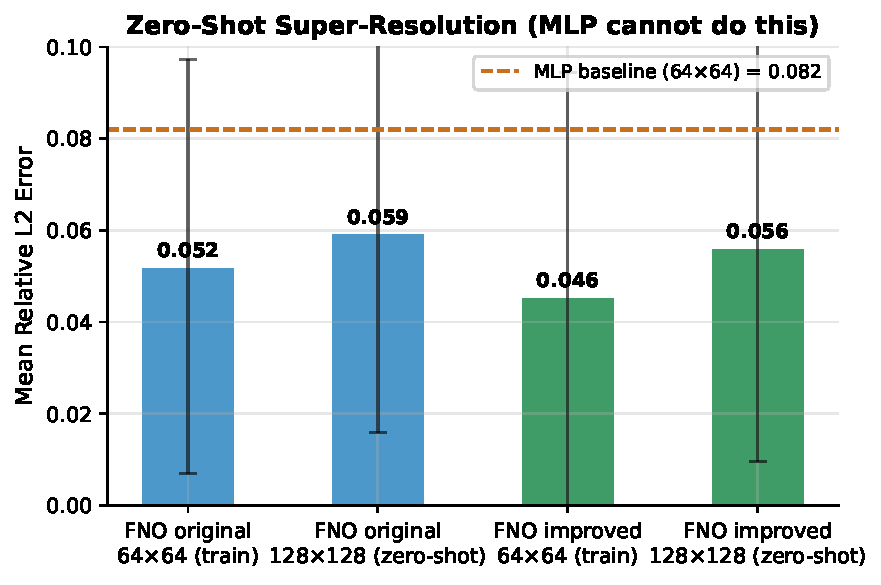
\includegraphics[width=0.58\textwidth]{../results/figures/fig3_superres.pdf}
\caption{Zero-shot super-resolution performance. Error bars show one standard deviation. The dashed line is the MLP baseline at its maximum resolution ($64\times64$).}
\end{figure}

% ─────────────────────────────────────────────────────────────────────────────
\section{Inference Speed}

We benchmarked inference speed on the training hardware (NVIDIA RTX PRO 6000) with batch size 1, reporting the median of 50 timed forward passes after 5 warm-up iterations. The FDM reference is the median of 20 SciPy sparse direct solves on CPU:

\begin{table}[H]
\centering
\caption{Inference speed per sample. FDM measured on CPU.}
\begin{tabular}{lrr}
\toprule
Model / Solver & Time (ms/sample) & Speedup vs.\ FDM \\
\midrule
FDM (reference) & 1030 & $1\times$ \\
MLP baseline    &  0.13 & $7740\times$ \\
FNO original    &  0.71 & $1443\times$ \\
\bottomrule
\end{tabular}
\end{table}

Both neural models are several orders of magnitude faster than the FDM reference. The MLP's lower inference latency is expected: it performs a single matrix--vector chain, whereas FNO computes 4 FFT pairs. Despite this, FNO's superior accuracy makes it the more practical operator surrogate.

% ─────────────────────────────────────────────────────────────────────────────
\section{Code Quality and Reproducibility}

The codebase is organised into four directories:
\begin{itemize}[nosep]
  \item \texttt{src/} --- \texttt{models.py} (\texttt{MLPBaseline}, \texttt{SpectralConv2d}, \texttt{FNO2d}), \texttt{train.py} (training loop; keeps the best-validation checkpoint), \texttt{evaluate.py}, \texttt{superres\_eval.py}, \texttt{benchmark\_speed.py}, \texttt{benchmark\_components.py}, \texttt{generate\_figures.py}.
  \item \texttt{configs/} --- \texttt{fno.yaml}, \texttt{fno\_improved.yaml}, \texttt{mlp.yaml}.
  \item \texttt{results/} --- one \texttt{run\_00x/} per model with its \texttt{eval\_metrics.json} (best epochs 92 / 99 / 198), plus \texttt{benchmark\_*.json} and \texttt{figures/}.
  \item \texttt{docs/} --- proposal, interim, and final reports.
\end{itemize}
A \texttt{pytest} suite covers model shapes, the relative-$L_2$ metric, and data loading; all results are committed. Training and evaluation reproduce with:
\begin{verbatim}
python3 src/train.py    --config configs/fno.yaml
python3 src/evaluate.py --config configs/fno.yaml \
    --checkpoint results/run_001/best_model.pt
python3 src/generate_figures.py
\end{verbatim}

% ─────────────────────────────────────────────────────────────────────────────
\section{Issues Encountered and Next Steps}

\subsection{Issues During Stage 1--2}
\begin{enumerate}[nosep]
  \item \textbf{GPU async timing}: Initial component profiling used \texttt{time.perf\_counter()} inside the GPU forward pass, measuring dispatch time rather than execution time. Fixed by calling a device-synchronisation primitive (\texttt{torch.cuda.synchronize()} on CUDA, \texttt{torch.mps.synchronize()} on Apple Silicon) before every timer read (implemented in \texttt{benchmark\_components.py}). The full layer-wise breakdown is deferred to the Stage 3 report.
  \item \textbf{Resolution mismatch at $128\times128$}: FNO retains only 12 Fourier modes; querying at $128\times128$ means every Fourier mode above the 12th is discarded, contributing to the $\sim14\%$ error increase in zero-shot evaluation.
  \item \textbf{MLP overfitting}: Despite GELU activations and weight decay, the MLP training curve showed larger train/val gap than FNO, suggesting the fixed-resolution architecture is less sample-efficient for this task.
\end{enumerate}

\subsection{Next Steps (Stage 3)}
\begin{enumerate}[nosep]
  \item \textbf{Physical interpretation}: Visualise prediction errors on specific samples; relate high-error cases to $\kappa$ field complexity.
  \item \textbf{Extended ablation}: Vary FNO modes (8, 12, 16, 20) and width (32, 64, 128) to map the accuracy--cost Pareto frontier.
  \item \textbf{Training resolution generalisation}: Train FNO directly at $128\times128$ and compare zero-shot vs.\ native $128\times128$ performance.
  \item \textbf{Error correlation}: Study whether per-sample error correlates with $\kappa$ heterogeneity (e.g., number of distinct regions, interface perimeter).
\end{enumerate}

% ─────────────────────────────────────────────────────────────────────────────
\begin{thebibliography}{9}
\bibitem{li2021fno}
  Z.\ Li et al., ``Fourier Neural Operator for Parametric Partial Differential Equations,'' \textit{ICLR}, 2021.

\bibitem{takamoto2022pdebench}
  M.\ Takamoto et al., ``PDEBench: An Extensive Benchmark for Scientific Machine Learning,'' \textit{NeurIPS}, 2022. DOI: 10.18419/darus-2986.
\end{thebibliography}

\end{document}
